\section{Auswertung}
\label{sec:Auswertung}

\begin{figure}
  \centering
  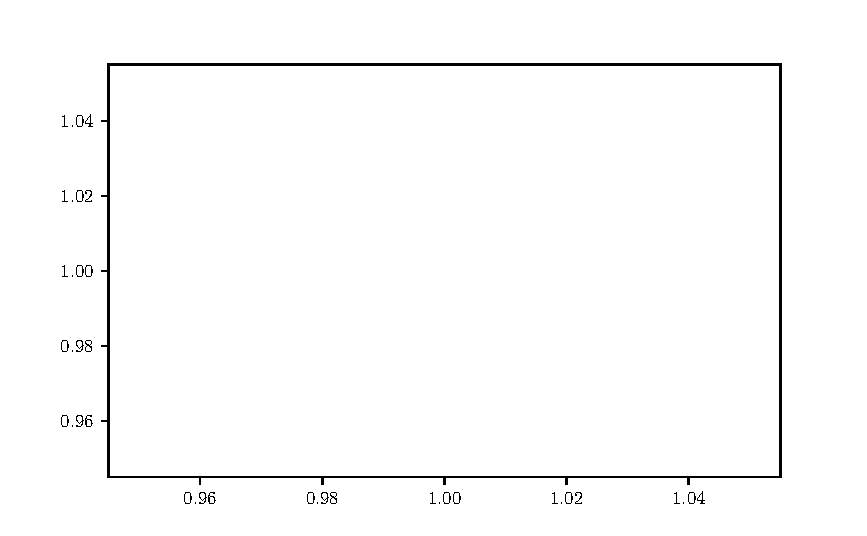
\includegraphics{plot.pdf}
  \caption{Plot}
  \label{fig:plot}
\end{figure}

\subsection{Bestimmung der Zeitkonstante}
Die Werte, die für die Bestimmung der Zeitkonstante $RC$ nötig sind, befinden sich in Tabelle \ref{table: }. %Tabelle
%Hier Tabelle einfügen
Die Zeitkonstante berechnet sich mittels Gleichung \eqref{eqn: RC} zu $RC = $. %Wert für RC 

\subsection{4b}
Die Kondensatorspannungen in Abhängigkeit von der Frequenz sind in Tabelle \ref{table: } dargstellt. %Tabelle
%Hier Tabelle einfügen
Die Zeitkonstante wird wieder durch \eqref{eqn: RC} berechnet. Es ergibt sich $RC = $. %Wert für RC

\subsection{4c}
In Tabelle \ref{table: } sind die Abstände der Nulldurchgänge der Spannung des Kondensators und der Spannung %Tabelle
des Generators in Abhängigkeit von der Frequenz dargestellt.
%Hier Tabelle einfügen
Mittels \eqref{eqn: RC} berechnet sich die Zeitkonstante zu $RC = $. %Wert für RC

\subsection{4d}
%Plots einfügen

%jeweils einzelne Formeln für RC in der Theorie angeben und hier erwähnen!